\chapter{Data Logging and Dashboard}\label{data_logging}

\section{Why do we need data?}

Data logging enables analysis of how internal variables change with time during a simulation. One might be interested in different variables from the system in question: messages frequency, food variation over time, agent deaths rate, etc.. Analysis also requires linking different simulation parameters with the data logged (e.g. the number of agents or the amount of food available). 

It is therefore important to setup a logging framework that structures data effectively and scales efficiently for large simulations. The below subsections will introduce the simulation parametrisation, followed by the different logging strategies (dumps and structured), and concluding with the logging interface and the analysis dashboard.

\section{Parametrisation}

First, it was important to enable an effective parametrisation of the simulation. A configuration interface was therefore set to abstract variables from the simulation environment. A configuration object would therefore be passed to the simulation environment instance, and it would define the following simulation parameters:

\begin{multicols}{2}
    \begin{enumerate}
        \item Agent count for each team
        \item Agent count for random agents
        \item Agent count for selfish agents
        \item Agent HP
        \item Agents per floor
        \item Amount of food on the platform
        \item Food per agent ratio (optional)
        \item Ticks per floor
        \item Total days
        \item Reshuffle period
    \end{enumerate}
\end{multicols}

The configuration parameters could then be written in a simple \texttt{json} file which would be parsed into a configuration object.

\section{General log dumps}

Following the configuration work, a general logger was setup. The general logger is basically a single shared logger between the different instances in the system (simulation, tower, agents, etc...). Each instance appends by default an identifier to a log line in the general logger log file (named \texttt{main.json}). Here is an example below:

\begin{verbatim}
{"agent_id":"dece1252","agent_type":"Team5","floor":3,"health":100,
"level":"info","msg":"Reporting agent state of team 5 agent","reporter":"agent"}

{"Floor:":7,"HP:":100,"Social motive:":"Altruist","agent_id":"2bfd3cfb",
"agent_type":"Team6","level":"info","msg":"Reporting agent state:","reporter":"agent"}

{"agent_id":"7873bb50","agent_type":"Team1","floor":5,"health":100,
"level":"info","msg":"Reporting agent state","reporter":"agent"}
\end{verbatim}

The general log dumps are unstructured - yet they enable agent teams to directly log custom states from their agents and use those in e.g. evolutionary algorithms or machine learning training.

\section{Structured logs}

The general log generates huge amounts of data and therefore was ineffective for data analysis and drawing conclusions easily from different simulations. Therefore, structured logs had to be introduced, where particular data is captured optimally to generate lightweight, understandable logs. After discussions with the agent teams and relating as fit to the problem, the following structured logs where included:

\begin{enumerate}
    \item \textbf{Food}: food available on the platform and food taken by agents.
    \item \textbf{Death}: agent death (including agent state at death time)
    \item \textbf{Messages}: receiver, sender, message type and content
    \item \textbf{Utility}: agent utility (including agent state)
    \item \textbf{Story}: a combination of the above logs in a sequential manner
\end{enumerate}

The agent state encapsulates by default the agent age, floor, HP, utility, and custom state (e.g. emotions or memory).

In the general log, custom agents could pass all sorts of information and therefore the log schema could not determined at compile time (which would be required for a visualisation dashboard). Structured logs have a well defined schema which does not depend on custom agents. For example, a food log will always take the following form:

\begin{verbatim}
{"day":2,"food":19,"level":"info","tick":222,"time":"2022-01-17T02:13:37Z"}
{"day":2,"food":0,"level":"info","tick":262,"time":"2022-01-17T02:13:37Z"}
{"day":3,"food":100,"level":"info","tick":321,"time":"2022-01-17T02:13:37Z"}
{"day":3,"food":90,"level":"info","tick":322,"time":"2022-01-17T02:13:37Z"}
\end{verbatim}

With structured logs set up, it is now possible to bundle logging into an interface and connect it to a visualisation tool.

\section{Logging interface}

It was important to set up logging such as structured loggers could be easily extended with new loggers, while preserving the ability to generate general logs. The following design has been adopted to encapsulate the simulation configuration and the loggers.

\begin{figure}[htb]
    \centering
    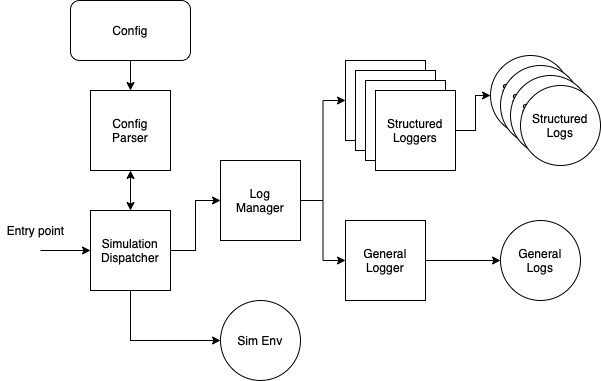
\includegraphics[width=0.8\linewidth]{003_data_logging/images/struct.png}
    \caption{Diagram showing how logging fits in the system}
    \label{fig:design_logging}
\end{figure}

The entry point to the simulation dispatcher was then linked to both the CLI as well as a server (with HTTP listeners) to support a browser-based dashboard.

\section{Dashboard}

With the logging interface, it was now possible to connect to the simulation entry point via a frontend and create simulations or visualise results. By design, the frontend had to support the following features:

\begin{enumerate}
    \item \textbf{Manage simulations}: easily navigate between different simulations
    \item \textbf{Create a simulation}: configure and run a new simulation
    \item \textbf{Numerical results}: display numerical outcomes such as total deaths or average utility
    \item \textbf{Graphical results}: display outcomes such as message types per agent type or food available per floor
\end{enumerate}

To encapsulate all these features, the dashboard was designed with the following structure:

\begin{figure}[htb]
    \centering
    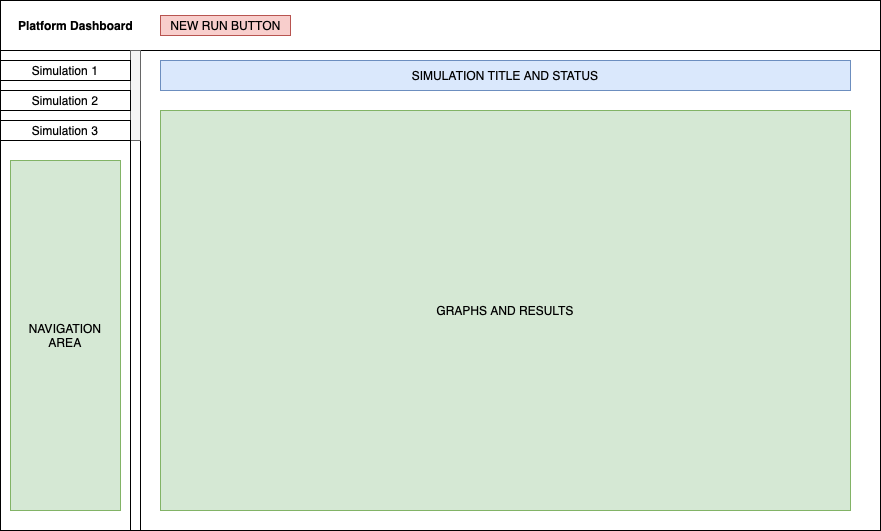
\includegraphics[width=\linewidth]{003_data_logging/images/design.png}
    \caption{Diagram showing the frontend design}
    \label{fig:design_ui}
\end{figure}

The "new simulation" button pops a configuration form where the user is able to fill in the different simulation parameters. The navigation area allows the user to switch between existing simulation results. Finally, numerical cards and different graph types have been included to visualise the results. The final frontend implementation can be tested online on \href{https://somas-2021-568r2.ondigitalocean.app}{https://somas-2021-568r2.ondigitalocean.app} or locally by following the guidelines on the \href{https://github.com/SOMAS2021/SOMAS2021#building-locally}{github repo}.